\chapter{Harmonogram realizacji projektu}
\label{cha:harmonogram}

\section{Etapy realizacji oraz wykres Gantta}
Proces realizacji aplikacji do zarządzania serwisem samochodowym został podzielony na kilka logicznych etapów, obejmujących analizę wymagań funkcjonalnych, projektowanie graficzne oraz techniczne, implementację interfejsu użytkownika, połączenie z bazą danych, testowanie i końcowe opracowanie dokumentacji projektowej.
Dzięki takiemu podziałowi możliwe było wdrażanie kolejnych funkcjonalności oraz szybka identyfikacja i eliminacja ewentualnych błędów na wczesnych etapach prac.

Realizacja przebiegała zgodnie z założonym planem. Niektóre zadania wymagały powrotu do wcześniejszych faz projektu - głównie w związku z wprowadzaniem nowych pomysłów, korektą koncepcji interfejsu lub dostosowaniem bazy danych do rozszerzonych wymagań funkcjonalnych.

Warto dodać, że niektóre działania były prowadzone równolegle, co pozwoliło usprawnić pracę nad projektem.
W celu zobrazowania harmonogramu, opracowano wykres Gantta (rys. \ref{fig:wykresGantta}), który przedstawia kolejne fazy projektu oraz przypisane im ramy czasowe.

\begin{figure}[H]
    \centering
    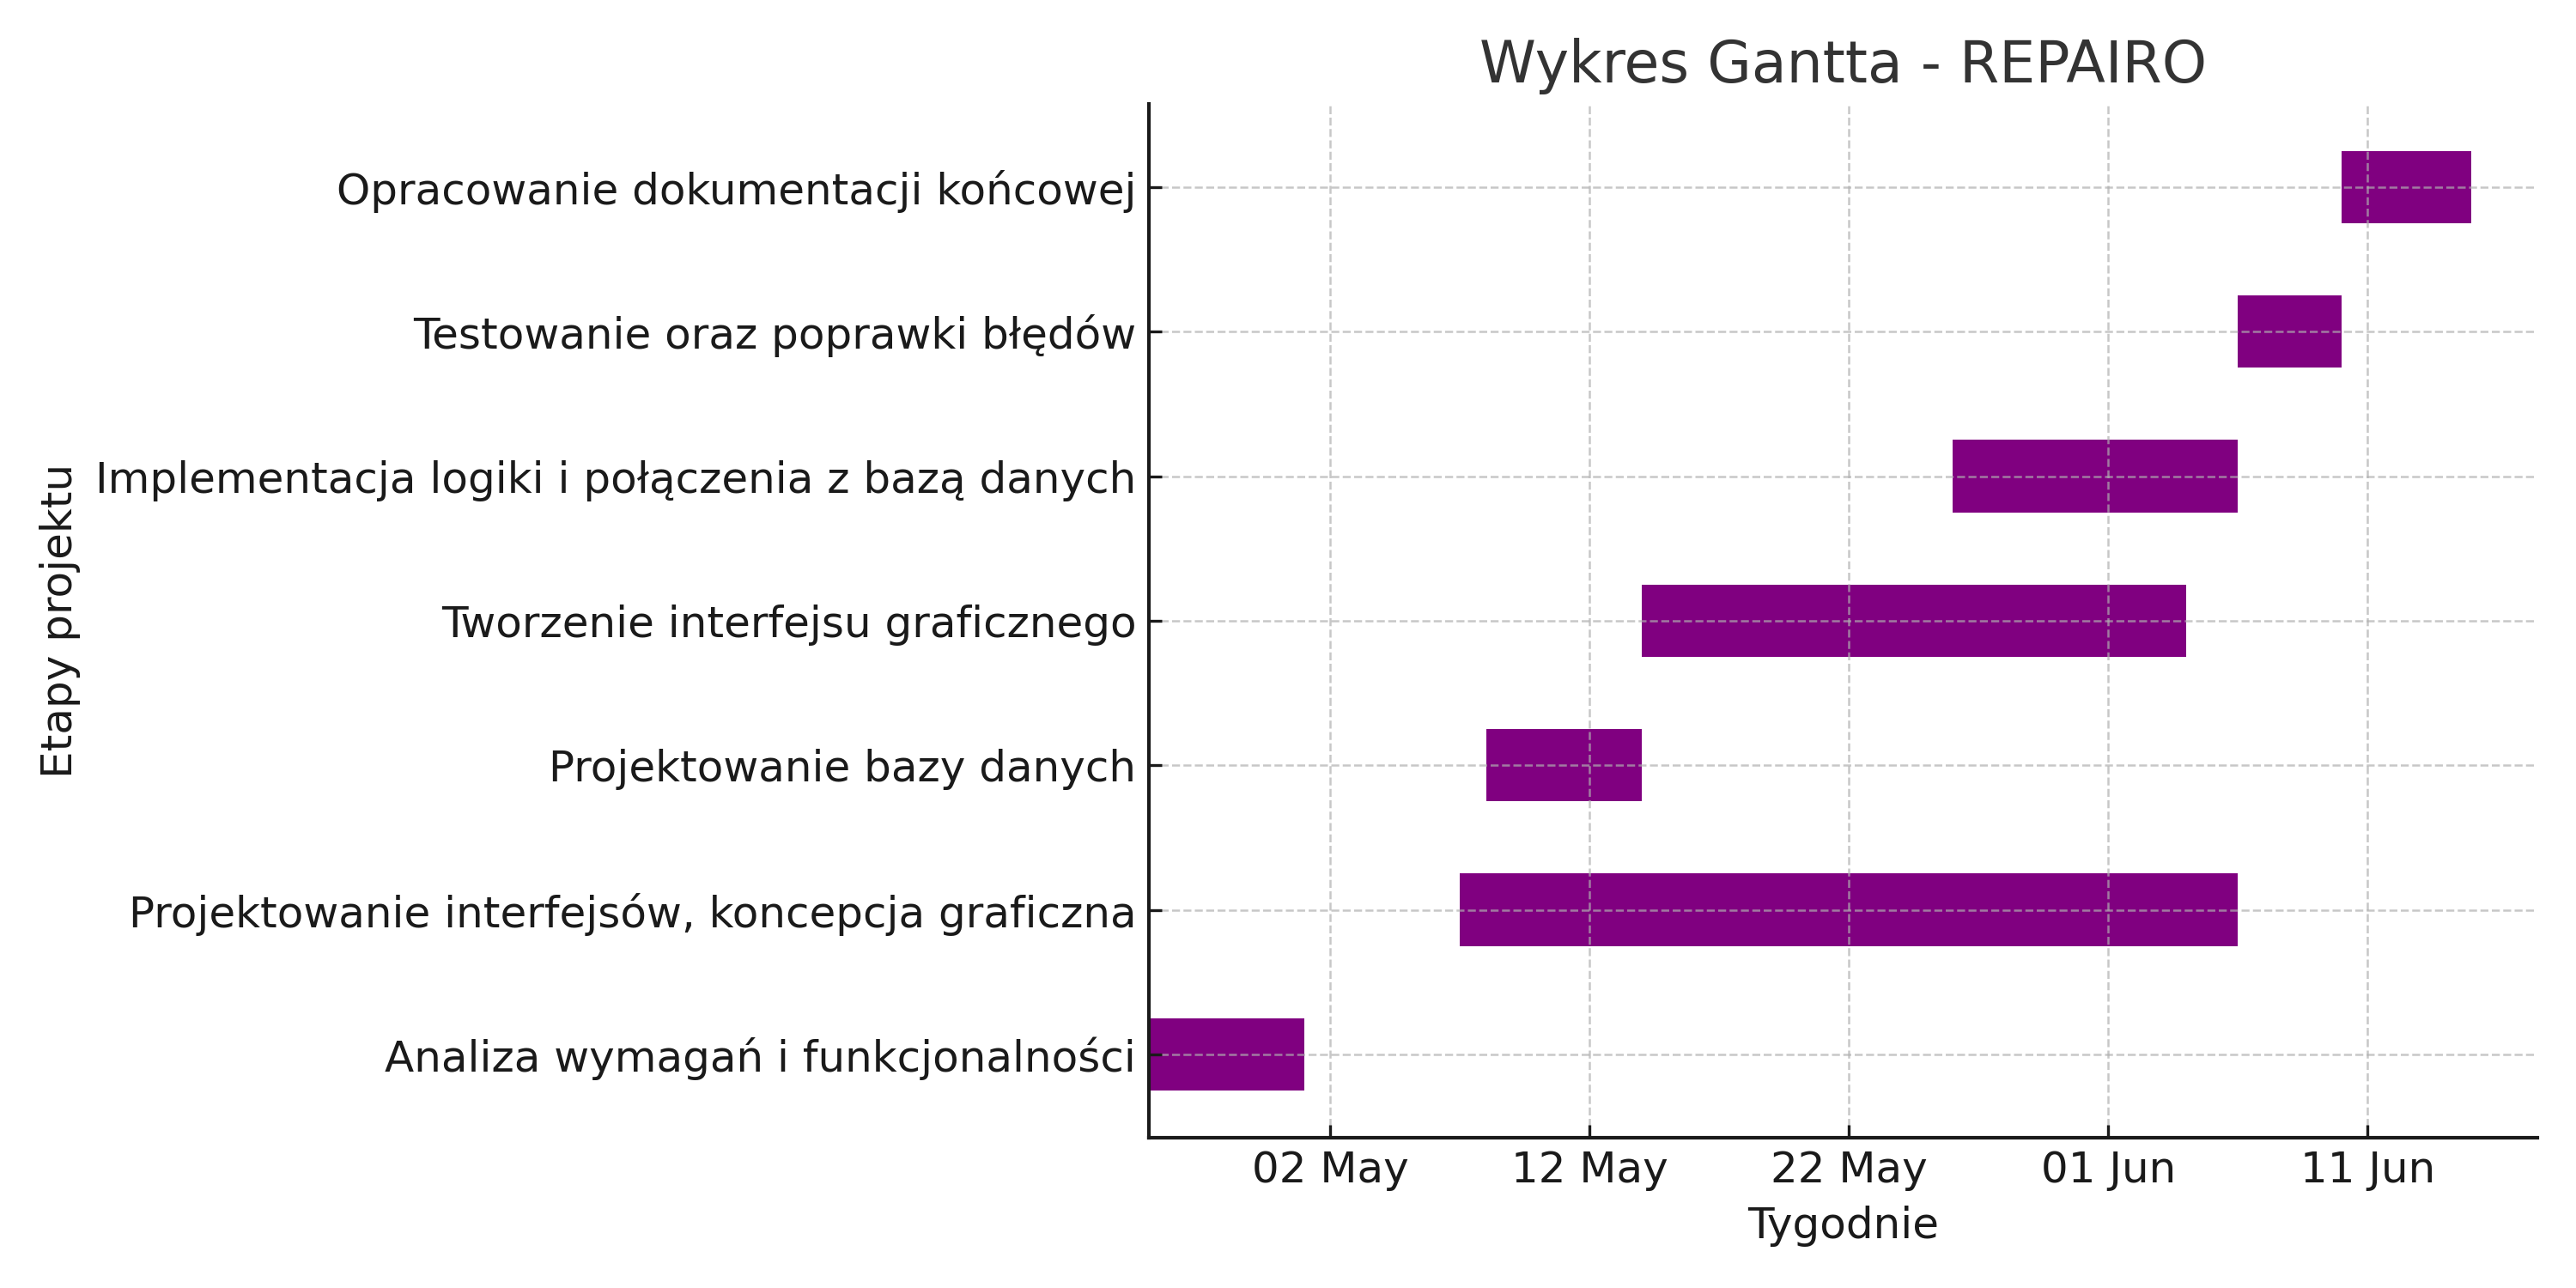
\includegraphics[width=\textwidth,height=0.8\textheight,keepaspectratio]{figures/wykres_gantta_repairo.png}
    \caption{Wykres Gantta REPAIRO}
    \label{fig:wykresGantta}
\end{figure}



\section{System kontroli wersji i repozytorium projektu}
W trakcie prac nad aplikacją wykorzystano system kontroli wersji \textbf{Git}, który umożliwił efektywne zarządzanie zmianami w kodzie. 
Cały projekt — kod źródłowy, pliki konfiguracyjne, struktura bazy danych oraz dokumentacja — został umieszczony na platformie \textbf{GitHub}.
\begin{center}
    \texttt{https://github.com/vLisek/SystemZarzadzaniaSerwisemSamochodowym}
\end{center}

Repozytorium zawiera ostateczną wersję projektu, okumentację projektowa oraz bazę danych. Zgodnie z wymaganiami, projekt dostępny będzie przez cały rok od daty oddania.